% This LaTeX was auto-generated from MATLAB code.
% To make changes, update the MATLAB code and export to LaTeX again.

\documentclass{article}

\usepackage[utf8]{inputenc}
\usepackage[T1]{fontenc}
\usepackage{lmodern}
\usepackage{graphicx}
\usepackage{color}
\usepackage{hyperref}
\usepackage{amsmath}
\usepackage{amsfonts}
\usepackage{epstopdf}
\usepackage[table]{xcolor}
\usepackage{matlab}

\sloppy
\epstopdfsetup{outdir=./}
\graphicspath{ {./le_4_1_8_images/} }

\begin{document}

\matlabheading{Algebra}

\begin{matlabcode}
syms s w
e1 = collect((s + 2*w) * (s + 3*w) * (s + 3*w + 1j*3*w) * (s + 3*w - 1j*3*w),s);
c1 = coeffs(e1,s); c1(end) = [];
S = s*eye(4);
A = [0, 1, 0, 0;...
     9*w^2, 0, 0, 2*w;...
     0, 0, 0, 1;...
     0, -2*w, -4*w^2, 0]; 
K = sym('k',[4 1]); C = [0 0 1 0];
e2 = collect(det(S - A + K*C),s);
c2 = coeffs(e2,s); c2(end) = [];
eqns = c1 == c2; 
Sol = solve(eqns,K); 
% Sol.k1
% Sol.k2
% Sol.k3
% Sol.k4
% clear; clc;
\end{matlabcode}


\matlabheading{system simulation (true-states)}

\begin{matlabcode}
omega = 2*pi/29.3; % orbital frequency [rad/s]
u = 1000 / (300 * omega^2) ; % input (F/(m*w^2)) [m/rad^2]
% state space representation [x; xdot; y; ydot]
A = [0, 1, 0, 0;...
     9*omega^2, 0, 0, 2*omega;...
     0, 0, 0, 1;...
     0, -2*omega, -4*omega^2, 0];
B = [0; 0; 0; 1]; C = [0, 0, 1, 0];
bryson_sattelite = @(t,x) A*x + B*u;

% simulation
y0 = [0; 0; 0; 0]; % initial states
tspan = [0 10]; % [days]
[t, y] = ode45(@(t,y) bryson_sattelite(t,y),tspan,y0);
\end{matlabcode}


\matlabheading{observers}

\begin{matlabcode}
% state observer 
K = [-71/2*omega; -181/2*omega^2; 11*omega; 55*omega^2];
mesh = @(x) interp1(t,y(:,3),x);
obs_bryson_sattelite = @(t,x) A*x + B*u + K*(mesh(t) - C*x);

% simulation 
y0 = rand([4 1]) * 500; % initial states
[to, yo] = ode45(@(t,y) obs_bryson_sattelite(t,y),tspan,y0); 

% error
for ii = 1:width(y)
    yq = interp1(t,y(:,ii),to);
    eq(:,ii) = yq - yo(:,ii);
end
\end{matlabcode}


\matlabheading{plots}

\begin{matlabcode}
figure(1); clf; tiledlayout(2,2)
ax(1) = nexttile; plot(t,y(:,1)/1e3,to,yo(:,1)/1e3,'LineWidth',2); box off
ylabel('$x$ [km]','Interpreter',"latex"); xlabel('$t$ [s]','Interpreter',"latex");
ax(2) = nexttile; plot(t,y(:,2)/1e3,to,yo(:,2)/1e3,'LineWidth',2); box off
ylabel('$\dot x$ [km/day]','Interpreter',"latex"); xlabel('$t$ [s]','Interpreter',"latex");
ax(3) = nexttile; plot(t,y(:,3)/1e3,to,yo(:,3)/1e3,'LineWidth',2); box off
ylabel('$y$ [km]','Interpreter',"latex"); xlabel('$t$ [s]','Interpreter',"latex");
ax(4) = nexttile; plot(t,y(:,4)/1e3,to,yo(:,4)/1e3,'LineWidth',2); box off;
ylabel('$\dot y$ [km/day]','Interpreter',"latex"); xlabel('$t$ [s]','Interpreter',"latex");
linkaxes(ax,'x'); clear ax;
% saving plots
textwidth = 14;
golden_ratio = (1 + sqrt(5)) / 2;
textheight = textwidth / golden_ratio;
figsize = [textwidth, textheight];

% Get latex font in ticks
h = findall(gcf,'Type','axes'); % An array if you have subplots
set(h, 'TickLabelInterpreter', 'latex')

% Set size and no crop
set(gcf, 'PaperUnits', 'centimeters', 'PaperSize', figsize);
set(gcf, 'PaperUnits', 'normalized', 'PaperPosition', [0, 0, 1, 1]);

print -dpdf ../doc/figures/ex418.pdf

figure(2); clf; tiledlayout(2,2)
ax(1) = nexttile; plot(to,eq(:,1)/1e3,'LineWidth',2); box off; xline(2.5,'--')
ylabel('$e_x$ [km]','Interpreter',"latex"); xlabel('$t$ [s]','Interpreter',"latex");
ax(2) = nexttile; plot(to,eq(:,2)/1e3,'LineWidth',2); box off; xline(2.5,'--')
ylabel('$e_{\dot x}$ [km/day]','Interpreter',"latex"); xlabel('$t$ [s]','Interpreter',"latex");
ax(3) = nexttile; plot(to,eq(:,3)/1e3,'LineWidth',2); box off; xline(2.5,'--')
ylabel('$e_y$ [km]','Interpreter',"latex"); xlabel('$t$ [s]','Interpreter',"latex");
ax(4) = nexttile; plot(to,eq(:,4)/1e3,'LineWidth',2); box off; xline(2.5,'--')
ylabel('$e_{\dot y}$ [km/day]','Interpreter',"latex"); xlabel('$t$ [s]','Interpreter',"latex");
linkaxes(ax,'x'); clear ax;
% saving plots
textwidth = 14;
golden_ratio = (1 + sqrt(5)) / 2;
textheight = textwidth / golden_ratio;
figsize = [textwidth, textheight];

% Get latex font in ticks
h = findall(gcf,'Type','axes'); % An array if you have subplots
set(h, 'TickLabelInterpreter', 'latex')

% Set size and no crop
set(gcf, 'PaperUnits', 'centimeters', 'PaperSize', figsize);
set(gcf, 'PaperUnits', 'normalized', 'PaperPosition', [0, 0, 1, 1]);

print -dpdf ../doc/figures/ex418_err.pdf
\end{matlabcode}
\begin{center}
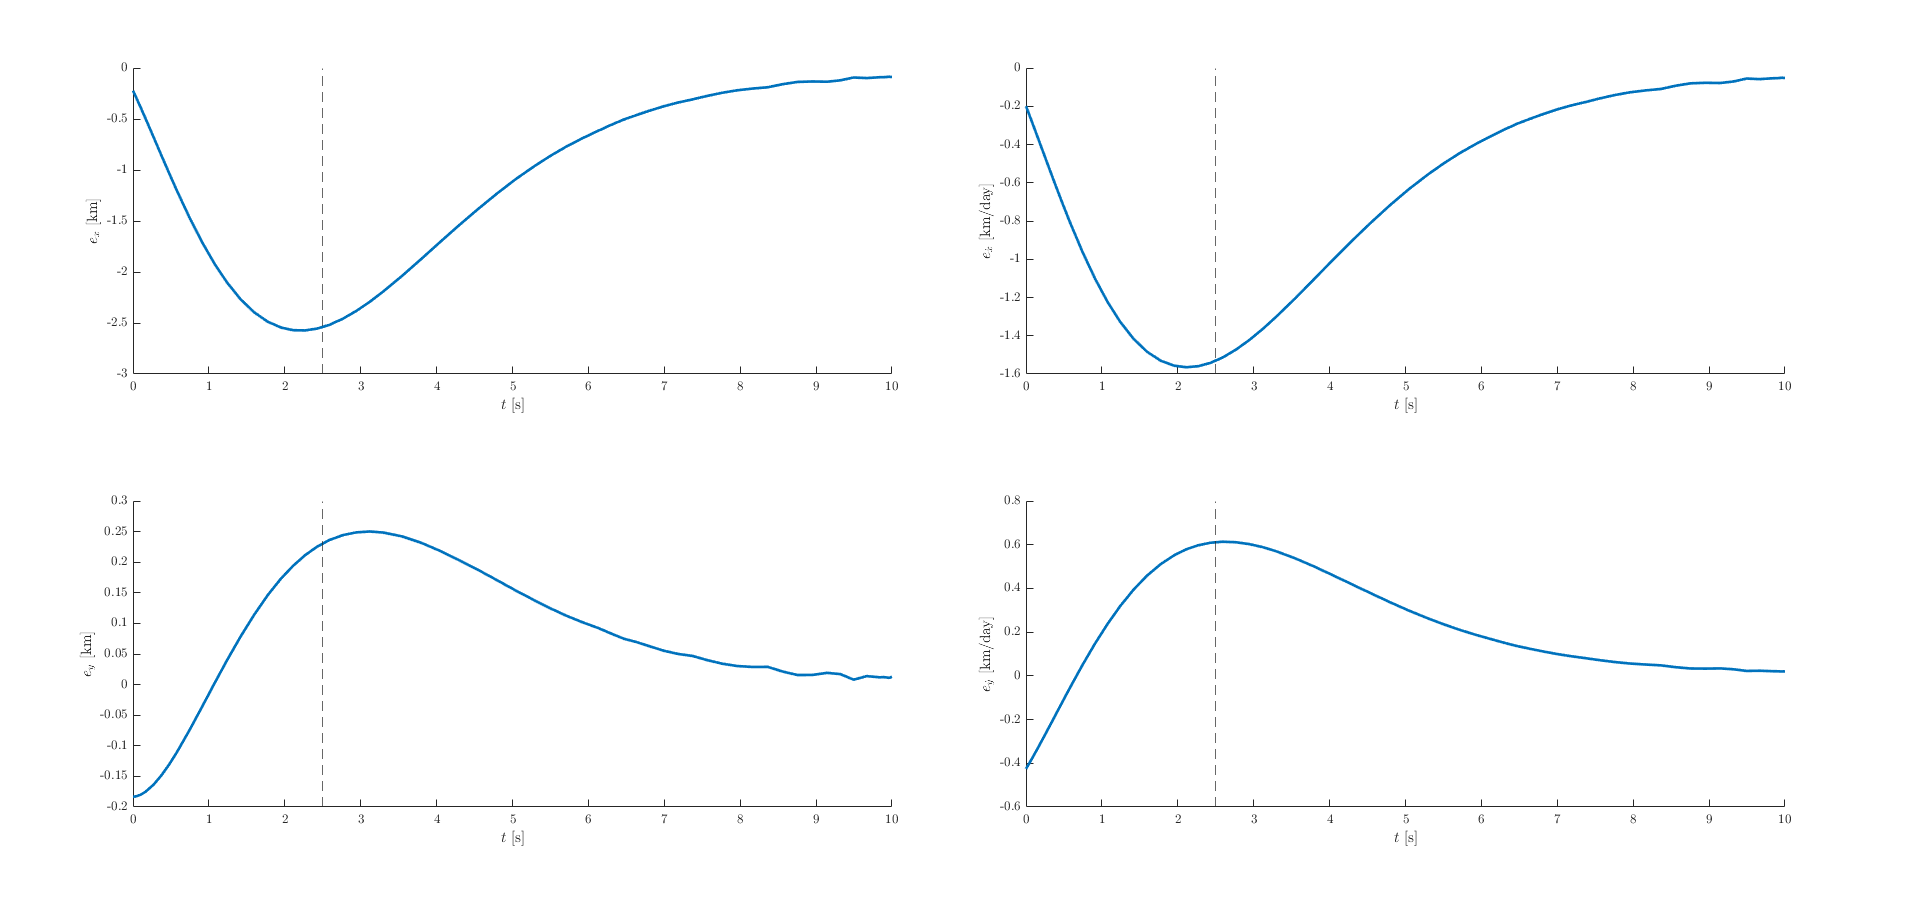
\includegraphics[width=\maxwidth{105.66984445559459em}]{figure_0.png}
\end{center}

\end{document}
